\documentclass[a4paper, 11pt]{article}
%\documentclass[pre,amsmath,aps,superscriptaddress,a4paper]{revtex4}
\usepackage{graphicx,xspace,units,subfigure}
\usepackage{float}
\usepackage{amsmath}
\usepackage{amssymb}
\usepackage[normalem]{ulem}
\usepackage{appendix}
\usepackage{hyperref}
\usepackage{setspace}
%\usepackage{helvet}
\usepackage{wrapfig}
\usepackage{eurosym}
%\usepackage{xcolor}
\usepackage{multirow}
\usepackage[dvipsnames]{xcolor}
\usepackage{comment}

% make a header
\usepackage{fancyhdr}
\pagestyle{fancy}
%\rhead{this is page \thepage}
%\chead{center of the footer!}
\renewcommand{\headrulewidth}{0.4pt}
%\renewcommand{\footrulewidth}{0.4pt}
\newlength\FHoffset
\setlength\FHoffset{0.1cm}
\addtolength\headwidth{2\FHoffset}
\fancyheadoffset{\FHoffset}

% Use sans serif throughout 
%\usepackage{fontspec}
%\renewcommand{\familydefault}{\sfdefault}
%\setsansfont{Helvetica}
  
\singlespacing
%\onehalfspacing
%\doublespacing
%\setstretch{1.1}

\usepackage{cite}          % writes reference [1,2,3] --> [1-3]
\usepackage{sectsty}     % center section without centering the subsections...
\sectionfont{\centering} % center section without centering the subsections...
\usepackage[font=small,labelfont=bf]{caption} % caption font size

%% Language and font encodings
\usepackage[english]{babel}
%\usepackage[utf8x]{inputenc}
%\usepackage[T1]{fontenc}

%% Sets page size and margins
\usepackage[a4paper,top=1.5cm,bottom=1.5cm,left=2cm,right=2cm]{geometry}
%\usepackage[a4paper,top=1.5cm,bottom=1.5cm,left=2cm,right=2cm,marginparwidth=1.75cm]{geometry}

\usepackage{color}
%\usepackage{helvet}
%\fontfamily{phv}
\usepackage{mdframed}

\newcommand{\be}{\begin{equation}}
\newcommand{\ee}{\end{equation}}

% \documentclass[a4paper, 11pt]{article}
% \usepackage[utf8]{inputenc}
% \usepackage{helvet}
% \fontfamily{phv}


% \usepackage{fullpage} % changes the margin





\begin{document}
\section*{Implementation of elasticity in sensory-growth rod-like organs}
\subsection*{Introduction}
This paper describes how to combine our formalism of active reorientations of growing rods with M. Gazzola's Cosserat filament integrator (see \emph{Gazzola RSOS 2018}). To do so, we decompose the stretch ($e$) to growth stretch ($e_g$) and elastic stretch ($e_e$): $e=e_e\cdot e_g$, following the mathematical formalism presented in A. Goriely's book (\emph{The Mathematics and Mechanics of Biological Growth, Springer 2017}). The mathematical decomposition of growth and elasticity originates from a distinct separation of timescales: the timescale of growth processes in plants (growth rates) is in the order of $10^4$ seconds, while their elastic relaxation times are of the order of $1-0.01$ seconds. We can therefore assume that the dynamics of a growing plant are in the quasi-static regime, in which the organ reaches its mechanical steady state for every growth step.

\begin{figure}[h!]
    \centering
    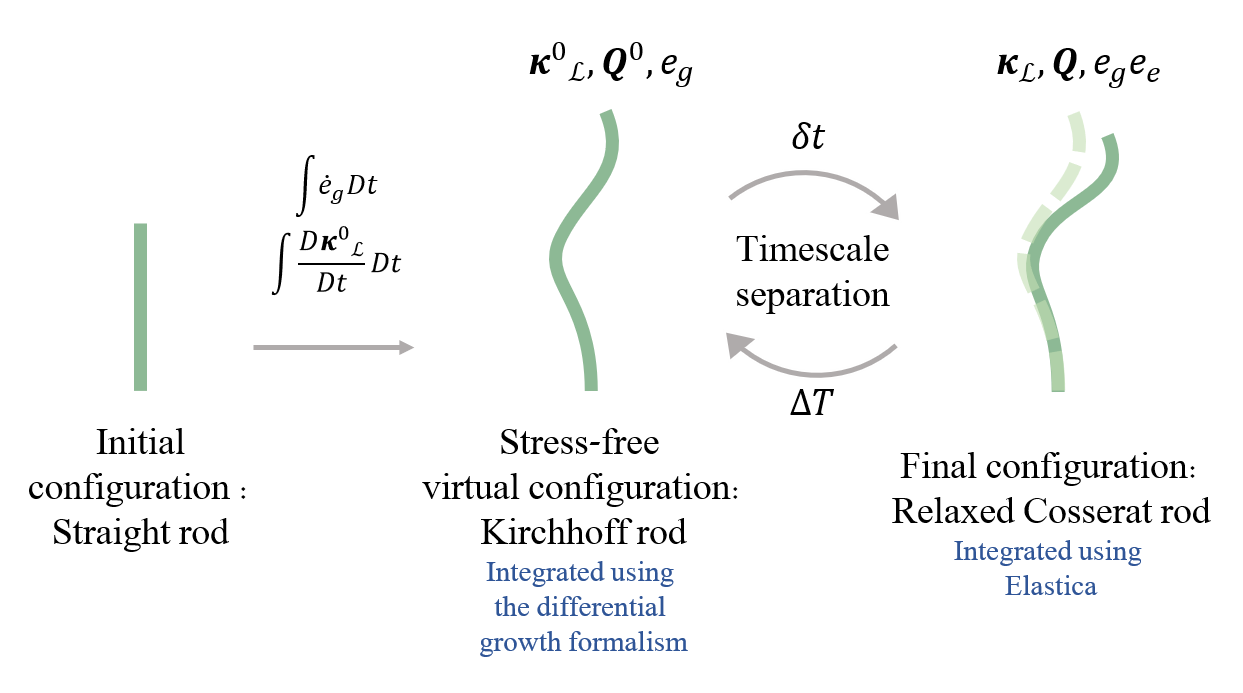
\includegraphics[width=0.80\textwidth]{growth_concept.png}
    \caption{\textbf{Integration scheme}. Starting from a straight rod, growth is implemented by updating the rest lengths and rest curvature vectors of the Cosserat rod according to the active growth model. One can think of rest lengths and curvatures as describing a referential stress-free virtual rod, as described in Goriely's book. Then, the Cosserat rod relaxes into its new stable mechanical state using Elatsica. The active growth step and passive mechnanical relaxation is iterated, and only the final relaxed configurations are collected.} \label{fig:fig1}
\end{figure}

\noindent Practically, we start from a straight rod clamped on one side, and let it grow. Growth is implemented by updating the rest lengths and rest curvature vectors of the Cosserat rod according to the active growth model. One can think of rest lengths and curvatures as describing a referential stress-free virtual rod, as described in Goriely's book. Then, the Cosserat rod relaxes into its new stable mechanical state using Elatsica. The active growth step and passive mechanical relaxation is iterated, and only the relaxed configurations of each growth step are collected.\\
To execute this integration scheme, several new basic functions must be written in the Cosserat rod class in Elastica:
\begin{itemize}
    \item \underline{Set growth parameters}: Defines the growth profile of the organ. Should be defined once before integration.
    \item \underline{Define tropisms}: Defines the active mechanisms that govern the dynamics of the rest curvture, based on our tropism model. Should be defined once before integration.
    \item \underline{Update growth}: Preforms a growth timestep: 
    \begin{itemize}
        \item \underline{Update differential growth vector:} Updates the differential growth vector based on the tropisms and the current state of the virtual and real rod. 
        \item \underline{Update virtual rod:} Updates the rest lengths and rest curvatures according to the given active growth mechanisms.
        \item \underline{Divide elements:} If an element grew above a given rest length threshold it is divided into two "daughter" elements. 
        \item \underline{Relaxation:} Runs Elastica until a mechanical steady state is reached. The steady state is defined by some integration criterion (e.g., rotational energy under 1e-12 for more than X timesteps).
    \end{itemize}
   
\end{itemize} 
We note that even though Elastica acts on a Cosserat rod, the active growth model doesn't include the existance of shear and its effect on active processes. Therefore, the implementation presented is correct to Kirchhoff rods, or Cosserat rods with small elastic strains ($|\boldsymbol{\sigma}_{\mathcal{L}}|\ll1$). \\
In the rest of the paper we go over each of the monetioned  functions in detail, using notations from \emph{Gazzola RSOS 2018}. 
\subsection*{Set growth parameters}
This function sets a growth rate profile along the organ: $\dot{e}_g(\hat{s},t)$, according to which the growth will occur. From now until stated otherwise, we neglect the index $t$, and treat all quantities with respect to the same growth time step. As a default, simple and smooth growth rate profile, we chose the logistic function, which requires 3 variables, $L_{gz}$, $\dot{E}_0$ and $m$:
\begin{equation}\label{eq:grp}
    \dot{e}_g(\hat{s})=\frac{\dot{E}_0}{1+\exp{\left(\frac{\hat{s}-(\hat{L}-L_{gz})}{L_{gz}/m}\right)}}
\end{equation}
where $\hat{s}_i=\sum_{j=1}^{i-1}\hat{\ell}_j$ is the rest arc-length of vertex $i$ (for $i>1$, as $\hat{s}_1=0$), and $\hat{L}=\hat{s}_{n+1}$.\\

\noindent \underline{Discretization:} The growth rate $\dot{e}_g$ is an elemental quantity ($\dot{e}_{g,1,...,n}$). Therefore, given a continuous function $\dot{e}_g(\hat{s})$, we define the growth rate of the $i$-th element as:
\begin{equation}
    \dot{e}_{g,i}=\frac{1}{\hat{\ell}_i}\int_{\hat{s}_i}^{\hat{s}_{i+1}}\dot{e}_g(\hat{s})d\hat{s}
\end{equation}
For the logistic function presented in Eq.~\ref{eq:grp}, this gives:
\begin{equation}
    \dot{e}_{g,i}=\frac{L_{gz}\dot{E}_0}{m\hat{\ell}_i}\ln{\left(\frac{1+\exp{\left(\frac{\hat{s}_{i+1}-(\hat{L}-L_{gz})}{L_{gz}/n}\right)}}{1+\exp{\left(\frac{\hat{s}_i-(\hat{L}-L_{gz})}{L_{gz}/n}\right)}}\right)}
\end{equation}
\begin{figure}[h!]
    \centering
    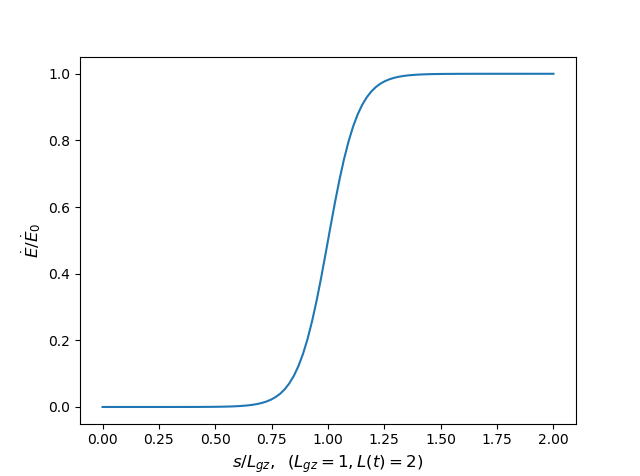
\includegraphics[width=0.60\textwidth]{growth_rate.png}
    \caption{Example of a growth rate profile, based on Eq.~\ref{eq:grp}, with $n=15$.}
\end{figure}


\newpage

\subsection*{Define tropisms}
This function sets the active growth processes that control the organ's reorientation, due to both internal processes and processes that depend on external stimuli (tropisms). This is done by defining the differential growth vector $\boldsymbol{\Delta}_{1,...,n-1}$ for each interior vertex using a sum of different competing processes:
\begin{equation}
    \boldsymbol{\Delta}_i=\sum_m\boldsymbol{\Delta}^m_i(\{x_j\})
\end{equation}
To each process different variables need to be given, marked above as $\{x_j\}$. If no variables are given for a certain process it is excluded. \\
The default tropisms are:
\begin{itemize}
    
    \item \underline{Directional tropism:} For a general directional tropism, the term requires a direction $\boldsymbol{d}$ and a tropic sensitivity $\lambda^d$. Then, term is: $\boldsymbol{\Delta}^d_i(\boldsymbol{d},\lambda^d)=\lambda^d\boldsymbol{d}$. One can see that the term doesn't depend on the element $i$.
    
    \item \underline{Gravitropism:} Following Elastica, the acceleration due to gravity point to the negative $y$ direction: $\boldsymbol{g}=-g\hat{\boldsymbol{y}}$. Since gravitropism is a negative tropism, the gravitropic term is: $\boldsymbol{\Delta}^g_i(\lambda^g)=(-\lambda^g)(-\hat{\boldsymbol{y}})=\lambda^g\hat{\boldsymbol{y}}$. One can see that the gravitropic term doesn't depend on the element $i$.
    
    \item \underline{Point tropism:} The point tropism receives a set of points $\{\boldsymbol{r}^p_j\}$ and a set of sensitivity functions $\{\lambda^p_j(\boldsymbol{r})\}$. Then, the point tropism term will have the shape:
    \begin{equation}
        \boldsymbol{\Delta}^p_{i}=\sum_j\boldsymbol{\Delta}^p_{i,j}=\sum_j\lambda^p_j(\boldsymbol{r}^p_j-\boldsymbol{r}_{i+1})\frac{\boldsymbol{r}^p_j-\boldsymbol{r}_{i+1}}{|\boldsymbol{r}^p_j-\boldsymbol{r}_{i+1}|}
    \end{equation}
    where we used the vertex $\boldsymbol{r}_{i+1}$ which is the interior vertex $\boldsymbol{r}^{(\text{int})}_{i}$. Notice that the locations of the points $\{\boldsymbol{r}^p_j\}$ may be updated at each growth time step, to enable pairwise interactions between organs.
    
    \item \underline{Non-local sensing:} All of the tropisms described thus far are local, that is, they sense the signal at their own locations. However, some organs sense signals only from their apex, or where the signal-specific sensors are located. The active tropic response is then non-local. This can be implemented in the code by introducing another variable to each tropism, that indicates at which vertex the signal is sensed, and how strong it is coupled. For example, if vertex $i$ grows according to the signal $m$ that is sensed in vertex $j$ with coupling $\mu_{ij}$, then the tropic term inherits the information from the $j$-th vertex according to:
    \begin{equation}
        \boldsymbol{\Delta}^{m,j}_{\mathcal{L},i}=\mu_{ij}\boldsymbol{\Delta}^{m}_{\mathcal{L},j}
    \end{equation}
    where the subscript $\mathcal{L}$ indicated that the vector is presented in the local coordinate frame. This notion can be extended to impulse response functions of signals by adding a time dependence in the coupling $\mu_{ij}(t-t_0)$, in which the signal was sensed at vertex $j$ at time $t_0$ (expressed in growth timesteps).
     
\end{itemize}

The default internal processes are:
\begin{itemize}
    \item \underline{Proprioception:} If we define the local curvature vector by: $\boldsymbol{\kappa}_{\mathcal{L},i}=(0,\kappa_i,\tau_i)$, then the proprioception term can be written as: $\boldsymbol{\Delta}^p_i(\gamma)=-\gamma\hat{\kappa}_i\boldsymbol{d}_{1,i}$, which uses the actual rest curvature, or $\boldsymbol{\Delta}^p_i(\gamma)=-\gamma\kappa^0_i\boldsymbol{d}_{1,i}$, which uses the intrinsic curvature. In \emph{Chelakkot 2017} the first form was taken, without apparent experimental or numerical validation.
    
    \item \underline{Circumnutation:} according to \emph{Bastein and Meroz 2015}, the circumnutation term is:
    \begin{equation}
    \boldsymbol{\Delta}^{c}_i(\omega_0)=\frac{R^0\kappa^0_i}{\dot{e}_{g,i}}\omega_0\boldsymbol{d}_{2,i}    
    \end{equation}
    where $R^0$ is the rest radius. Notice that circumnutation doesn't occur if the rest curvature is zero.
\end{itemize}

\subsection*{Update growth}
The basic principle is to decompose the total stretch in the organ into growth stretch ($e_g$) and an elastic stretch ($e_e$):
\begin{equation}
    e=e_e\cdot e_g
\end{equation}
Referring to the re-scaling of segment properties in Gazzola's 2018 paper, the growth stretch $e_g$ does not change the area or curvature of the segment, and adds mass to the segment. Therefore, the following relations hold:
\begin{equation}
    ds=e\cdot d\hat{s}=e_e\cdot e_gd\hat{s}\;,\;
    R=\frac{\hat{R}}{\sqrt{e_e}}\;,\;
    A=\frac{\hat{A}}{e_e}\;,\;
    I=\frac{\hat{I}}{e_e^2}\;,\;
    B=\frac{\hat{B}}{e_e^2}\;,\;
    S=\frac{\hat{S}}{e_e}\;,\;
    \kappa_{\mathcal{L}}=\frac{\hat{\boldsymbol{\kappa}}_{\mathcal{L}}}{e_e}
\end{equation}
The mass of the segment will be:
\begin{equation}
    dm=\rho \pi R^2 ds=e_g\rho\pi\hat{R}^2 d\hat{s}
\end{equation}
\\
\noindent \underline{Quasi-static integration:} There a distinct separation of timescales in our problem: the timescale of growth processes in plants is in the order of $10^4$ seconds, while their elastic relaxation times are of the order of $1-0.01$ seconds. We can therefore assume that the dynamics of a growing plant are in the quasi-static regime, in which the organ has reaches the steady state for every step of growth. One can thus choose to implement growth either by growing the plant in time-steps which are dictated by the elastic relaxation process (that is, growth takes place when the energy minimizes to a certain minimal threshold), or continuously growing the organ at a very slow rate. \\

\noindent \underline{Body forces ramp:} The code should run smoothly and simulate quasi static growth after an initial relaxation to external forces. Since the initial state of the organ is assumed to be a straight rod, the initial relaxation to gravity may take a while due to oscillations and their damping by dissipation. This relaxation initialization can be reduced by adding the external forces in a quasi-static manner.\\

\noindent \underline{Segment division:} For a constant profile of growth rates along the organ, after long periods of time the growth stretch $e_g$ will inevitably reach high values (for example around the apex), for which the discrete segments approximation is no longer be valid. Therefore, a "segment division" should be implemented above a certain threshold of local growth stretch $e_g$. In this division, the segment is to be split in half, while both halves should retain all of its properties but its length:
\begin{equation}
    ds_i=ds_{i,1}+ds_{i,2}
\end{equation}
The propagation of the local coordinates should be updated accordingly.
\\

\noindent \underline{Current plan:} write a code (and a wrapper?) that: 
\begin{itemize}
    \item Implements various growth rate functions $\dot{e}_g(s,t)$ (exponential, apical flat and apical Gaussian). 
    \item Limits growth time-step by maximal growth velocity (apical velocity): $v_{\text{max}}=\int_0^{L(t)}\dot{e}_g(s,t)ds$ 
    \item Divides segments that elongate over a certain threshold ($d\hat{s}>ds_{\text{max}}$). This includes the calculation of the local coordinate system (Q) of the two parts of the divided segments, and will probably require recalculations of the Voronoi regions.
    \item Propagates intrinsic curvature (and twist) according to the active growth model.
\end{itemize}



\newpage

\subsection*{Element division}
In a growing rod, if an element (or an edge) grows above a certain threshold, we need to divide it into two distinct elements. Using the code of Gazzola's lab, the division can be implemented by breaking down the element, $\boldsymbol{\ell}_i=\boldsymbol{r}_{i+1}-\boldsymbol{r}_{i}$, into two new elements (see Fig.~\ref{fig:fig1}):
\begin{equation}
    \boldsymbol{\ell}_i=\boldsymbol{\ell}_{i,1}+\boldsymbol{\ell}_{i,2}
\end{equation}


\begin{figure}[h!]
    \centering
    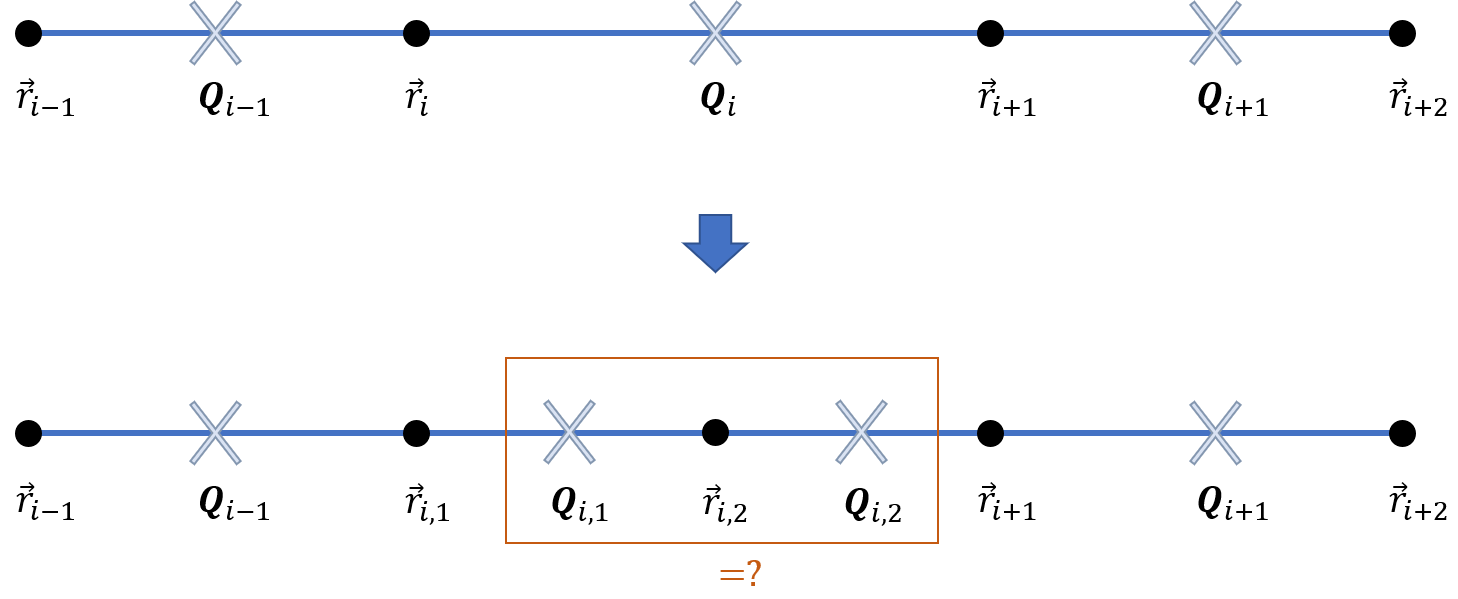
\includegraphics[width=0.80\textwidth]{seg_div.png}
    \caption{\textbf{Segment division}. One must demand continuity in $\boldsymbol{r}$, $\boldsymbol{Q}$ and $\boldsymbol{a}$ in order to find the corrects values for the characteristics of the new "daughter" elements. } \label{fig:fig1}
\end{figure}
\noindent Each segment has a variety of local variables, that are defined either pointwise on the vertices, for example the segments physical location $\vec{r}_i$ and mass $m_i$, as an edge property, such as the tangent vector $\boldsymbol{t}$ or strain $\hat{\boldsymbol{\sigma}}^i_{\mathcal{L}}$, or on the interior vertex, for example the inextensible curvature $\hat{\boldsymbol{\kappa}}_\mathcal{L}$. 
\noindent For simplicity, we assume that the rest length of the segment splits to two equal lengths, or:
\begin{equation}
\hat{\ell}_{i,1}=\hat{\ell}_{i,1}=\frac{1}{2}\hat{\ell}_i    
\end{equation}
and that the elastic stretch $e_i$ and the shear vector $\vec{\sigma}_i$ remain constant on the two "daughter" segments:
\begin{equation}
    e_{i,1}=e_{i,2}=e_{i}\;\;\;,\;\;\; \boldsymbol{\sigma}^{i,1}_\mathcal{L}=\boldsymbol{\sigma}^{i,2}_\mathcal{L}=\boldsymbol{\sigma}^i_\mathcal{L}
\end{equation}
To properly find the curvatures and the local material frames of the new segments, one must demand that the surrounding quantities remain constant, that is, that $\boldsymbol{r}_{i+1}$ and $\boldsymbol{r}_{i}=\boldsymbol{r}_{i,1}$ don't change, and neither do $\boldsymbol{Q}_{i-1}$ and $\boldsymbol{Q}_{i+1}$.\\
We start the condition on the local coordinate frames. We notice that one can write the relation between $\boldsymbol{Q}_{i-1}$ and $\boldsymbol{Q}_{i+1}$ using the Rodrigues formula twice \textcolor{blue}{(notice that it's not the same formula in the article, a minus needs to be added)}:
\begin{equation}\label{eq:Q1}
    \boldsymbol{Q}_{i+1}=\exp\left(-{\hat{\mathcal{D}}_i\hat{\boldsymbol{\kappa}}^i_\mathcal{L}}\right)\boldsymbol{Q}_i=\exp\left(-{\hat{\mathcal{D}}_i\hat{\boldsymbol{\kappa}}^i_\mathcal{L}}\right)\exp\left(-\hat{\mathcal{D}}_{i-1}\hat{\boldsymbol{\kappa}}^{i-1}_\mathcal{L}\right)\boldsymbol{Q}_{i-1}
\end{equation}
Where:
\begin{equation}
    \hat{\mathcal{D}}_i=\frac{1}{2}(\hat{\ell}_{i+1}+\hat{\ell}_{i})
\end{equation}
In a similar manner, after the division we have:
\begin{equation}\label{eq:Q2}
    \boldsymbol{Q}_{i+1}=\exp\left(-\hat{\mathcal{D}}_{i,2}\hat{\boldsymbol{\kappa}}^{i,2}_\mathcal{L}\right)\exp\left(-\hat{\mathcal{D}}_{i,1}\hat{\boldsymbol{\kappa}}^{i,1}_\mathcal{L}\right)\exp\left(-\hat{\mathcal{D}}'_{i-1}\hat{\boldsymbol{\kappa}}^{i-1}_\mathcal{L}\right)\boldsymbol{Q}_{i-1}
\end{equation}
where we notice that:
\begin{equation}
    \hat{\mathcal{D}}_{i-1}=\frac{1}{2}(\hat{\ell}_{i}+\hat{\ell}_{i-1})\neq\hat{\mathcal{D}}'_{i-1}=\frac{1}{2}(\hat{\ell}_{i,1}+\hat{\ell}_{i-1})=\frac{1}{2}(\frac{1}{2}\hat{\ell}_{i}+\hat{\ell}_{i-1})
\end{equation}
Eq.~\ref{eq:Q1} and Eq.~\ref{eq:Q2} give the continuity condition on the local coordinate frame:
\begin{equation}
    \exp\left(-{\hat{\mathcal{D}}_i\hat{\boldsymbol{\kappa}}^i_\mathcal{L}}\right)\exp\left(-\hat{\mathcal{D}}_{i-1}\hat{\boldsymbol{\kappa}}^{i-1}_\mathcal{L}\right)=\exp\left(-\hat{\mathcal{D}}_{i,2}\hat{\boldsymbol{\kappa}}^{i,2}_\mathcal{L}\right)\exp\left(-\hat{\mathcal{D}}_{i,1}\hat{\boldsymbol{\kappa}}^{i,1}_\mathcal{L}\right)\exp\left(-\hat{\mathcal{D}}'_{i-1}\hat{\boldsymbol{\kappa}}^{i-1}_\mathcal{L}\right)
\end{equation}
or explicitly:
\begin{align}\label{eq:Q_f}
    \exp\left(-{\frac{1}{2}(\hat{\ell}_{i+1}+\hat{\ell}_{i})\hat{\boldsymbol{\kappa}}^i_\mathcal{L}}\right)\exp\left(-\frac{1}{2}(\hat{\ell}_{i}+\hat{\ell}_{i-1})\hat{\boldsymbol{\kappa}}^{i-1}_\mathcal{L}\right)&=\nonumber\\
    =\exp\left(-\frac{1}{2}(\hat{\ell}_{i+1}+\frac{1}{2}\hat{\ell}_{i})\hat{\boldsymbol{\kappa}}^{i,2}_\mathcal{L}\right)&\exp\left(-\frac{1}{2}\hat{\ell}_i\hat{\boldsymbol{\kappa}}^{i,1}_\mathcal{L}\right)\exp\left(-\frac{1}{2}(\frac{1}{2}\hat{\ell}_{i}+\hat{\ell}_{i-1})\hat{\boldsymbol{\kappa}}^{i-1}_\mathcal{L}\right)
\end{align}
We can see from Eq.~\ref{eq:Q_f} that we have 2 unknowns: $\hat{\boldsymbol{\kappa}}^{i,1}_\mathcal{L}$ and $\hat{\boldsymbol{\kappa}}^{i,2}_\mathcal{L}$. To find them, we now add the requirement that the spatial vectors $\boldsymbol{r}_{i+1} $ and $\boldsymbol{r}_{i}=\boldsymbol{r}_{i,1}$ remain unchanged. To do so, we look at the expression for the strain vector:
\begin{equation}
    \boldsymbol{\sigma}^i_\mathcal{L}=\boldsymbol{Q}_i\left(\frac{\partial \boldsymbol{r}_i}{\partial \hat{s}}-\boldsymbol{d}^i_3\right)
\end{equation}
Multiplying from the left by $\boldsymbol{Q}^T_i$ and integrating by $\hat{s}$ give:
\begin{equation}\label{eq:r_1}
    \boldsymbol{r}_{i+1}=\left(\boldsymbol{Q}^T_i\boldsymbol{\sigma}^i_\mathcal{L}+\boldsymbol{d}^i_3\right)\hat{\ell}_i+\boldsymbol{r}_{i}
\end{equation}
Or:
\begin{equation}
    \boldsymbol{\ell}_i=\left(\boldsymbol{Q}^T_i\boldsymbol{\sigma}^i_\mathcal{L}+\boldsymbol{d}^i_3\right)\hat{\ell}_i
\end{equation}
In a similar fashion, we can now write the relation between $\boldsymbol{r}_{i+1} $ and $\boldsymbol{r}_{i}=\boldsymbol{r}_{i,1}$ after the division:
\begin{align}
    \boldsymbol{r}_{i+1}&=\boldsymbol{\ell}_{i,2}+\boldsymbol{\ell}_{i,1}+\boldsymbol{r}_{i}\nonumber\\
    &=\left(\boldsymbol{Q}^T_{i,2}\boldsymbol{\sigma}^{i,2}_\mathcal{L}+\boldsymbol{d}^{i,2}_3\right)\hat{\ell}_{i,2}+\left(\boldsymbol{Q}^T_{i,1}\boldsymbol{\sigma}^{i,1}_\mathcal{L}+\boldsymbol{d}^{i,1}_3\right)\hat{\ell}_{i,1}+\boldsymbol{r}_{i}=\nonumber\\
    &=\left(\left(\boldsymbol{Q}^T_{i,2}+\boldsymbol{Q}^T_{i,1}\right)\boldsymbol{\sigma}^{i}_\mathcal{L}+\boldsymbol{d}^{i,2}_3+\boldsymbol{d}^{i,1}_3\right)\frac{\hat{\ell}_{i}}{2}+\boldsymbol{r}_{i}\label{eq:r_2}
\end{align}
where in the last equation we used the assumption of a constant strain vector.
Equating Eq.~\ref{eq:r_1} and Eq.~\ref{eq:r_2} gives the continuity condition on the rod's position:
\begin{equation}\label{eq:cond_pos}
    \boldsymbol{Q}^T_i\boldsymbol{\sigma}^i_\mathcal{L}+\boldsymbol{d}^i_3=\frac{1}{2}\left(\left(\boldsymbol{Q}^T_{i,2}+\boldsymbol{Q}^T_{i,1}\right)\boldsymbol{\sigma}^{i}_\mathcal{L}+\boldsymbol{d}^{i,2}_3+\boldsymbol{d}^{i,1}_3\right)
\end{equation}
Using the Einstein notation, we notice that:
\begin{equation}\label{eq:EIN}
   \boldsymbol{Q}^T\boldsymbol{\sigma}_\mathcal{L}+\boldsymbol{d}_3=\boldsymbol{Q}^T_{ij} \boldsymbol{\sigma}_{\mathcal{L},j}+\boldsymbol{Q}_{ij}\delta_{i,3}=\boldsymbol{Q}_{ji} \boldsymbol{\sigma}_{\mathcal{L},j}+\boldsymbol{Q}_{ij}\delta_{i,3}=\boldsymbol{Q}_{ij}\left(\boldsymbol{\sigma}_{\mathcal{L},i}+\delta_{i,3}\right)
\end{equation}
Plugging Eq.~\ref{eq:EIN} into Eq.~\ref{eq:cond_pos} gives a simplified condition:
\begin{equation}\label{eq:Q12}
    \boldsymbol{Q}_i=\frac{1}{2}\left(\boldsymbol{Q}_{i,2}+\boldsymbol{Q}_{i,1}\right)\;\;.
\end{equation}
Writing both sides of Eq.~\ref{eq:Q12} using $\boldsymbol{Q}_{i-1}$ and the Rodrigues formula gives the relation:
\begin{align}\label{eq:Qr1}
    &\exp\left(-\frac{1}{2}(\hat{\ell}_{i}+\hat{\ell}_{i-1})\hat{\boldsymbol{\kappa}}^{i-1}_\mathcal{L}\right)=\nonumber\\
    &=\frac{1}{2}\left(\exp\left(-\frac{1}{2}\hat{\ell}_i\hat{\boldsymbol{\kappa}}^{i,1}_\mathcal{L}\right)\exp\left(-\frac{1}{2}(\frac{1}{2}\hat{\ell}_{i}+\hat{\ell}_{i-1})\hat{\boldsymbol{\kappa}}^{i-1}_\mathcal{L}\right)+
    \exp\left(-\frac{1}{2}(\frac{1}{2}\hat{\ell}_{i}+\hat{\ell}_{i-1})\hat{\boldsymbol{\kappa}}^{i-1}_\mathcal{L}\right)\right)
\end{align}
We now remind the reader that if $A$ is a matrix and $a,b$ are scalars, then $e^{aA}e^{bA}=e^{(a+b)A}$. Hence, multiplying Eq.~\ref{eq:Qr1} from the right by $\exp\left(\frac{1}{2}(\frac{1}{2}\hat{\ell}_{i}+\hat{\ell}_{i-1})\hat{\boldsymbol{\kappa}}^{i-1}_\mathcal{L}\right)$ gives: 
\begin{equation}\label{eq:k1_1}
    \exp\left(-\frac{1}{4}\hat{\ell}_{i}\hat{\boldsymbol{\kappa}}^{i-1}_\mathcal{L}\right)=\frac{1}{2}\left(\exp\left(-\frac{1}{2}\hat{\ell}_i\hat{\boldsymbol{\kappa}}^{i,1}_\mathcal{L}\right)+1\right)
\end{equation}
which gives us $\hat{\boldsymbol{\kappa}}^{i,1}_\mathcal{L}$:
\begin{equation}\label{eq:kappa1}
    \hat{\boldsymbol{\kappa}}^{i,1}_\mathcal{L}=-\frac{2}{\hat{\ell}_{i}}\ln{\left(2\exp\left(-\frac{1}{4}\hat{\ell}_{i}\hat{\boldsymbol{\kappa}}^{i-1}_\mathcal{L}\right)-1\right)}
\end{equation}
Inserting the resulting $\hat{\boldsymbol{\kappa}}^{i,1}_\mathcal{L}$ into Eq.~\ref{eq:Q_f} will give us $\hat{\boldsymbol{\kappa}}^{i,2}_\mathcal{L}$. We begin by multiplying Eq.~\ref{eq:Q_f} from the right by $\exp\left(\frac{1}{2}(\frac{1}{2}\hat{\ell}_{i}+\hat{\ell}_{i-1})\hat{\boldsymbol{\kappa}}^{i-1}_\mathcal{L}\right)$. This gives:
\begin{align}\label{eq:Q_fd}
    \exp\left(-{\frac{1}{2}(\hat{\ell}_{i+1}+\hat{\ell}_{i})\hat{\boldsymbol{\kappa}}^i_\mathcal{L}}\right)\exp\left(-\frac{1}{4}\hat{\ell}_{i}\hat{\boldsymbol{\kappa}}^{i-1}_\mathcal{L}\right)&=\nonumber\\
    =\exp\left(-\frac{1}{2}(\hat{\ell}_{i+1}+\frac{1}{2}\hat{\ell}_{i})\hat{\boldsymbol{\kappa}}^{i,2}_\mathcal{L}\right)&\exp\left(-\frac{1}{2}\hat{\ell}_i\hat{\boldsymbol{\kappa}}^{i,1}_\mathcal{L}\right)
\end{align}
Inserting Eq.~\ref{eq:k1_1} into Eq.~\ref{eq:Q_fd} gives:
\begin{align}\label{eq:Q_fd2}
    \exp\left(-{\frac{1}{2}(\hat{\ell}_{i+1}+\hat{\ell}_{i})\hat{\boldsymbol{\kappa}}^i_\mathcal{L}}\right)\exp\left(-\frac{1}{4}\hat{\ell}_{i}\hat{\boldsymbol{\kappa}}^{i-1}_\mathcal{L}\right)&=\nonumber\\
    =\exp\left(-\frac{1}{2}(\hat{\ell}_{i+1}+\frac{1}{2}\hat{\ell}_{i})\hat{\boldsymbol{\kappa}}^{i,2}_\mathcal{L}\right)&\left(2\exp\left(-\frac{1}{4}\hat{\ell}_{i}\hat{\boldsymbol{\kappa}}^{i-1}_\mathcal{L}\right)-1\right)
\end{align}
To isolate $\hat{\boldsymbol{\kappa}}^{i,2}_\mathcal{L}$, we multiply Eq.~\ref{eq:Q_fd2} by the inverse of the exponentials in the correct order. This gives:
\begin{equation}
    \label{eq:Q_fd3}
    \exp{\left(\frac{1}{2}(\hat{\ell}_{i+1}+\frac{1}{2}\hat{\ell}_{i})\hat{\boldsymbol{\kappa}}^{i,2}_\mathcal{L}\right)}
    =\left(2-\exp{\left(\frac{1}{4}\hat{\ell}_{i}\hat{\boldsymbol{\kappa}}^{i-1}_\mathcal{L}\right)}\right) \exp{\left(\frac{1}{2}(\hat{\ell}_{i+1}+\hat{\ell}_{i})\hat{\boldsymbol{\kappa}}^i_\mathcal{L}\right)}
\end{equation}
or:
\begin{equation}
    \hat{\boldsymbol{\kappa}}^{i,2}_\mathcal{L}
    =\frac{4}{2\hat{\ell}_{i+1}+\hat{\ell}_i}\ln{\left(\left(2-\exp{\left(\frac{1}{4}\hat{\ell}_{i}\hat{\boldsymbol{\kappa}}^{i-1}_\mathcal{L}\right)}\right) \exp{\left(\frac{1}{2}(\hat{\ell}_{i+1}+\hat{\ell}_{i})\hat{\boldsymbol{\kappa}}^i_\mathcal{L}\right)}\right)}
\end{equation}
Then, the rest curvatures of the new segments are known, and the local coordinate frames can be found using the Rodrigues formula:
\begin{equation}
    \boldsymbol{Q}_{i,1}=\exp\left(-\frac{1}{2}(\frac{1}{2}\hat{\ell}_{i}+\hat{\ell}_{i-1})\hat{\boldsymbol{\kappa}}^{i-1}_\mathcal{L}\right)\boldsymbol{Q}_{i-1}\;\;,\;\;\boldsymbol{Q}_{i,2}=\exp\left(-\frac{1}{2}\hat{\ell}_i\hat{\boldsymbol{\kappa}}^{i,1}_\mathcal{L}\right)\boldsymbol{Q}_{i,1}
\end{equation}


\noindent Special attention should be given to the last element: Since the last node doesn't have a corresponding curvature, only the curvature of the new node is missing.  The continuity in $\boldsymbol{r}$ gives us the required $\hat{\boldsymbol{\kappa}}^{i,1}_\mathcal{L}$, as expressed in Eq.~\ref{eq:kappa1}. 

\noindent \textcolor{blue}{This derivation is true for the real curvature. A parallel calculation must be done for the virtual rod, where the propagation in arc length of the local coordinate frame is done with the intrinsic (rest) curvature rather than the real one.}




\newpage

\subsection*{Growth rate coupling}
In real plants, the total growth rate $\dot{\epsilon}$ is coupled to external stresses on the organ $\sigma$, as described by the Lockhart model:
\begin{equation}
    \dot{\epsilon}\propto (P-Y-\sigma) \Theta (P-Y-\sigma)
\end{equation}
where $P$ is the plant's Turgur pressure, $Y$ is the cell wall's yield stress, and $\Theta$ is the Heavyside function. 
We therefore see that growth can stop if the external stresses $\sigma$ are high enough. \\
To implement this coupling in our model, I suggest to project this relation to the local tangent direction.  Then, the local growth rate would be written by:
\begin{equation}
    \dot{E}(s,t)=\dot{E}_0(s,t)\cdot\left(1-\frac{\sigma_3}{\sigma_{\text{max}}}\right)
\end{equation}
where $\sigma_3$ is the stretch along $\hat{T}$ (or $\hat{\mathcal{D}}_3$), and $\dot{E}_0(s,t)$ is the predefined growth rate without stresses on the segment.\\
\subsection*{Aging effects}
To insert aging effects, one must give a time dependence to both the bending modulus of the organ $B=B(s,t)$, and to the radius, as radial growth is possible in long times. At first, we ignore these effects completely.

\subsection*{Growth model - intrinsic curvature and actual curvature}
By definition, active growth processes affect the shape of the organ by changing its intrinsic curvature and torsion. Then, an elastic relaxation of the form of the organ will give its actual form. However, signals' directions should be related to the actual form of the organ, as the organs' sensors are assumed to respond to the local stimuli (neglecting memory phenomena). If we mark the intrinsic curvature by $\kappa_0$, the actual curvature by $\kappa$, and the intrinsic torsion as $\tau_0=\partial \phi_0/\partial s$, our growth dynamics can be written as:\\
\begin{equation}\label{eq:prop}
        \frac{1}{\dot{E}}\frac{D(R\kappa_0)}{Dt}=\vec{\Delta}\cdot\hat{N}=\vec{\lambda}\cdot\hat{N}-\gamma \kappa_0
\end{equation}
\begin{equation}
    \frac{\kappa_0}{\dot{E}} \frac{D(R\phi_0)}{Dt}=\vec{\Delta}\cdot\hat{B}=\vec{\lambda}\cdot\hat{B}
\end{equation}
where $\vec{\lambda}$ is the local sensitivity vector, parallel to the direction of a certain stimulus, and $\gamma$ is the proprioception coefficient. In contrast, in Chelakkot2017 a simpler formalism was assumed for the curvature's dynamics (as they delt only with 2-d organs):
\begin{equation}\label{eq:prop2}
        \frac{1}{\dot{E}}\frac{D(R\kappa_0)}{Dt}=\vec{\lambda}\cdot\hat{N}-\gamma \kappa
\end{equation}
One can see that here the proprioception term is written using the actual curvature. Since the microscopic biological details of proprioception are unknown, both models are possible.\\ 

\noindent This form does not include relaxation of the intrinsic curvature and torsion to the actual curvature and torsion. However, plants do relax internal strains using growth (see Goldstein and Goriely, Phys. Rev. E 74, 010901(R), 2006). This relaxation can either arise from a process related to the axial growth, in which case it should be implemented in our model, or from a radial growth processes, which is yet to be implemented. Assuming a strain relaxation process does takes place in the axial direction, the growth model may take the form:
\begin{equation}\label{eq:relax}
        \frac{1}{\dot{E}}\frac{D(R\kappa_0)}{Dt}=\vec{\lambda}\cdot\hat{N}+\gamma (\kappa-\kappa_0)
\end{equation}
\begin{equation}
     \frac{D\tau_0}{Dt}=\frac{\partial}{\partial s} \left(\frac{\dot{E}}{R\kappa_0}\vec{\lambda}\cdot\hat{B}\right)+\gamma\frac{\dot{E}}{R} (\tau-\tau_0)
\end{equation}
We note that we replaced the proprioception term with the strain relaxation process. We now turn to try and compare the three growth models presented.





\end{document}


